\documentclass[11pt]{aghdpl}
% \documentclass[en,11pt]{aghdpl}  % praca w języku angielskim

% Lista wszystkich języków stanowiących języki pozycji bibliograficznych użytych w pracy.
% (Zgodnie z zasadami tworzenia bibliografii każda pozycja powinna zostać utworzona zgodnie z zasadami języka, w którym dana publikacja została napisana.)
\usepackage[english,polish]{babel}

%%% fix for \lll
\let\babellll\lll
\let\lll\relax

% Użyj polskiego łamania wyrazów (zamiast domyślnego angielskiego).
\usepackage{polski}

\usepackage[utf8]{inputenc}
	
\newcommand*{\captionsource}[2]{%
  \caption[{#1}]{%
    #1%
    \\\hspace{\linewidth}%
    \textbf{Źródło:} #2%
  }%
}

% dodatkowe pakiety

\usepackage{mathtools}
\usepackage{amsfonts}
\usepackage{amsmath}
\usepackage{amsthm}
\usepackage{amssymb}
\usepackage{float}
\usepackage{epstopdf}

\numberwithin{equation}{section}

% --- < bibliografia > ---

\usepackage[
style=numeric,
sorting=none,
%
% Zastosuj styl wpisu bibliograficznego właściwy językowi publikacji.
language=autobib,
autolang=other,
% Zapisuj datę dostępu do strony WWW w formacie RRRR-MM-DD.
urldate=iso8601,
% Nie dodawaj numerów stron, na których występuje cytowanie.
backref=false,
% Podawaj ISBN.
isbn=true,
% Nie podawaj URL-i, o ile nie jest to konieczne.
url=false,
%
% Ustawienia związane z polskimi normami dla bibliografii.
maxbibnames=3,
% Jeżeli używamy BibTeXa:
backend=bibtex
]{biblatex}

\usepackage{csquotes}
% Ponieważ `csquotes` nie posiada polskiego stylu, można skorzystać z mocno zbliżonego stylu chorwackiego.
\DeclareQuoteAlias{croatian}{polish}

\addbibresource{bibliografia.bib}

% Nie wyświetlaj wybranych pól.
%\AtEveryBibitem{\clearfield{note}}


% ------------------------
% --- < listingi > ---

% Użyj czcionki kroju Courier.
\usepackage{courier}

\usepackage{listings}
\lstloadlanguages{TeX}

\lstset{
	literate={ą}{{\k{a}}}1
           {ć}{{\'c}}1
           {ę}{{\k{e}}}1
           {ó}{{\'o}}1
           {ń}{{\'n}}1
           {ł}{{\l{}}}1
           {ś}{{\'s}}1
           {ź}{{\'z}}1
           {ż}{{\.z}}1
           {Ą}{{\k{A}}}1
           {Ć}{{\'C}}1
           {Ę}{{\k{E}}}1
           {Ó}{{\'O}}1
           {Ń}{{\'N}}1
           {Ł}{{\L{}}}1
           {Ś}{{\'S}}1
           {Ź}{{\'Z}}1
           {Ż}{{\.Z}}1,
	basicstyle=\footnotesize\ttfamily,
}

% ------------------------

\AtBeginDocument{
	\renewcommand{\tablename}{Tabela}
	\renewcommand{\figurename}{Rys.}
}

% ------------------------
% --- < tabele > ---

\usepackage{array}
\usepackage{tabularx}
\usepackage{multirow}
\usepackage{booktabs}
\usepackage{makecell}
\usepackage[flushleft]{threeparttable}

% defines the X column to use m (\parbox[c]) instead of p (`parbox[t]`)
\newcolumntype{C}[1]{>{\hsize=#1\hsize\centering\arraybackslash}X}


%---------------------------------------------------------------------------

\author{Marcin Kowalczyk}
\shortauthor{M. Kowalczyk}

\titlePL{System wizyjny śledzący obiekty wykorzystujący ruchomą kamerę zrealizowany w oparciu o heterogeniczny układ Zynq.}
\titleEN{An object tracking vision system using a moving camera implemented in a Zynq heterogeneous device.}


\shorttitlePL{System wizyjny realizujący śledzenie z ruchomą kamerą.}
\shorttitleEN{An object tracking vision system with moving camera.}

\thesistype{Praca dyplomowa inżynierska}

\supervisor{dr inż. Tomasz Kryjak}

\degreeprogramme{Automatyka i Robotyka}

\date{2016}

\department{Katedra Automatyki i Inżynierii Biomedycznej}

\faculty{Wydział Elektrotechniki, Automatyki,\protect\\[-1mm] Informatyki i Inżynierii Biomedycznej}

\acknowledgements{Serdecznie dziękuję \dots tu ciąg dalszych podziękowań np. dla promotora, żony, sąsiada itp.}


\setlength{\cftsecnumwidth}{10mm}

%---------------------------------------------------------------------------
\setcounter{secnumdepth}{4}
\brokenpenalty=10000\relax

\begin{document}

\titlepages

% Ponowne zdefiniowanie stylu `plain`, aby usunąć numer strony z pierwszej strony spisu treści i poszczególnych rozdziałów.
\fancypagestyle{plain}
{
	% Usuń nagłówek i stopkę
	\fancyhf{}
	% Usuń linie.
	\renewcommand{\headrulewidth}{0pt}
	\renewcommand{\footrulewidth}{0pt}
}

\setcounter{tocdepth}{2}
\tableofcontents
\clearpage

\chapter{Wstęp}
\label{cha:wstep}

\section{Cel pracy}
\label{sec:celpracy}

Celem pracy jest stworzenie demonstratora systemu wizyjnego do śledzenia obiektów, przy czym zakłada się, że kamera zamontowana jest na głowicy obrotowej. Praca inżynierska obejmuje skompletowanie, we współpracy z opiekunem, stanowiska testowego składającego się z głowicy ruchomej, kamery, platformy obliczeniowej oraz wskaźnika. Należy przeprowadzić analizę oraz weryfikację różnych koncepcji śledzenia, biorąc pod uwagę skuteczność oraz możliwość implementacji sprzętowej lub sprzętowo-programowej. Wybrane rozwiązanie zostało zaimplementowane, uruchomione i przetestowane w sprzęcie. Wyjście z modułu śledzenia stanowi podstawę do wypracowania pozycjonowania głowicy obrotowej, takiego, aby utrzymać obiekt w środku kadru oraz oznaczyć go wskaźnikiem.

\section{Wprowadzenie}
\label{sec:wprowadzenie}

Automatyczne śledzenie z pomocą kamery jest wykorzystywane m.in. w zagadnieniach związanych z bezpieczeństwem, inwigilacją lub w zastosowaniach wojskowych. Jest ściśle powiązane z wykrywaniem oraz identyfikacją obiektów. Świadczy to o złożoności tego zagadnienia. Śledzenie różni się od innych algorytmów przetwarzania obrazów głównie tym, że musimy wykorzystywać informacje pochodzące z więcej niż jednego kadru. Uwydatnia się to szczególnie, kiedy kamera rejestruje kilka obiektów podobnych do śledzonego. Jeśli zadaniem jest obserwacja jednego konkretnego obiektu, to aby go wyróżnić musimy wykorzystać położenie śledzonego obiektu w poprzednich ramkach \cite{VT}. Znaczące problemy w śledzeniu obiektów mogą być spowodowane zmianą orientacji celu oraz dużą jego szybkością w porównaniu do częstotliwości rejestrowania klatek. W przypadku kamery umieszczonej na głowicy błędy mogą być dodatkowo spowodowane rozmyciem obrazu w trakcie poruszania układu. Istnieją liczne algorytmy służące śledzeniu elementu na obrazach z kamery. Są to m.in:
\begin{itemize}
\item{Śledzenie przez detekcję}
\item{Mean-shift}
\item{Filtr cząsteczkowy}
\item{KLT}
\end{itemize}
Algorytmy te zostaną dokładniej omówione w kolejnym rozdziale pracy.

\section{Zawartość pracy}
\label{sec:zawartoscpracy}

W rozdziale \dots
\chapter{Algorytmy}
\label{cha:algorytmy}

W rozdziale tym omówione zostaną algorytmy śledzenia. Rozważymy również możliwość oraz skuteczność ich implementacji sprzętowej i sprzętowo-programowej.

\section{Śledzenie przez detekcję}
\label{sec:sledzenieprzezdetekcje}

Jest to najłatwiejszy możliwy algorytm śledzenia. Polega on na detekcji obiektu i określeniu jego położenia (np. poprzez wyznaczenie środka ciężkości). Algorytm ten jest efektywny tylko, gdy w kadrze znajduje się maksymalnie jeden wyznaczony obiekt. Ograniczenie to możemy obejść przez zastosowanie dodatkowo algorytmu indeksacji. Wtedy musimy zdecydować który z wyznaczonych obiektów jest tym właściwym. Możemy np. śledzić element znajdujący się najbliżej (mający największą powierzchnię w kadrze). Efektywność implementacji programowo-sprzętowej zależy w większości od wykorzystanego algorytmu detekcji, i/lub segmentacji. Algorytm detekcji na podstawie koloru będzie łatwy i szybki do zaimplementowania, a algorytm bazujący na współczynnikach kształtu  wymagać będzie dużo więcej pracy i zasobów.

\section{Mean-shift}
\label{sec:meanshift}

Algorytm ten bazuje na statystycznej metodzie poszukiwania lokalnego maksimum rozkładu prawdopodobieństwa. Polega on na wyznaczeniu maksymalnej wartości prawdopodobieństwa w aktualnym oknie wokół punktu startowego. W celu zastosowania tego algorytmu do śledzenia obiektu należy przedstawić obraz jako rozkład prawdopodobieństwa. W tym celu każdemu pikselowi przypisuje się wartość prawdopodobieństwa. Można to zrobić np. na podstawie koloru, przypisując kolorom wartość prawdopodobieństwa, lub histogramu, porównując histogram otoczenia piksela z histogramem obiektu \cite{CMS}. Jeśli prawdopodobieństwo obliczone zostaje tylko na podstawie koloru, dobre wyniki można uzyskać, gdy \cite{CMS}:
\begin{itemize}
\item Obiekt ma jednolitą barwę.
\item Występują bardzo małe zmiany oświetlenia.
\item W kadrze nie ma obiektów podobnych do śledzonego.
\item Kolor tła znacznie różni się od koloru obiektu.
\item Obiekt nie zostaje całkowicie zasłonięty.
\end{itemize}
\paragraph*{}
Algorytm ten ma następujący przebieg:
\begin{enumerate}
\item Wybierz rozmiar okna.
\item Wybierz początkowe położenie(środek) okna.
\item Wyznacz położenie maksimum wartości prawdopodobieństwa w oknie.
\item Przesuń okno, aby wyznaczone maksimum było jego środkiem.
\item Powtarzaj kroki 3 i 4, aż algorytm będzie zbieżny.
\end{enumerate}
\paragraph*{}
Punktem startowym dla każdego kolejnego obrazu z kamery jest pozycja obiektu w poprzednim obrazie. Poszukiwanie maksymalnej wartości prawdopodobieństwa odbywa się w następujący sposób:
\begin{itemize}
\item Obliczamy moment zerowy.
\begin{equation}
M_{00}=\sum\limits_{x}\sum\limits_{y}l(x,y)
\end{equation}
\item Obliczamy moment pierwszy dla osi poziomej.
\begin{equation}
M_{10}=\sum\limits_{x}\sum\limits_{y}x \cdot l(x,y)
\end{equation}
\item Obliczamy moment pierwszy dla osi pionowej.
\begin{equation}
M_{01}=\sum\limits_{x}\sum\limits_{y}y \cdot l(x,y)
\end{equation}
\item Obliczamy środek rozkładu prawdopodobieństwa w danym oknie.
\begin{equation}
x_c=\frac{M_{10}}{M_{00}}
\end{equation}
\begin{equation}
y_c=\frac{M_{01}}{M_{00}}
\end{equation}
\end{itemize}
Gdzie \(l(x,y)\) jest wartością prawdopodobieństwa dla piksela \((x,y)\)\cite{BCV}.

%\paragraph*{}
%Można wykorzystać przykładowe jądra:
%\begin{itemize}
%\item Płaskie
%\[K(x)=\begin{cases}1 & \text{dla } x \leqslant R \\ 0 & \text{dla } x>R \end{cases}\]
%\item Gaussowskie
%\[K(x)=\frac{1}{2\pi}\mathrm{e}^{-\frac{1}{2} \cdot |x|^2}\]
%\end{itemize}
%\paragraph*{}
%Dla zestawu \(n\) punktów w 2-wymiarowej przestrzeni estymacja gęstości jądra z jądrem K(x) i promieniem %#\(h\) wynosi:
%#\[f_K(x)=\frac{1}{nh^2} \cdot \sum\limits_{i=1}^{n}K(\frac{x-x_i}{h})\]

\section{Filtr cząsteczkowy}
\label{sec:filtrczasteczkowy}

Filtr cząsteczkowy inaczej nazywany jest sekwencyjną metodą Monte Carlo. Punktem startowym algorytmów tego typu jest model obiektu w postaci równań stanu \cite{Mukhtar}:
\begin{equation}
\label{eq:PF_state}
x_k=Ax_{k-1}+Bu_k+w_{k-1}
\end{equation}
\begin{equation}
y_k=Cx_k+v_k
\end{equation}
\(x_k\) jest ukrytym, prawdziwym stanem obiektu.\newline
\(y_k\) jest obserwowanym stanem obiektu.\newline
\(w_{k-1}\) jest zmienną losową o rozkładzie normalnym reprezentującą szum przetwarzania.\newline
\(v_k\) jest zmienną losową o rozkładzie normalnym reprezentującą szum pomiarowy.\newline
%Jeśli obiekt porusza się ze stałą prędkością, przyjąć należy następujące macierze \(A\) i \(B\):
%\begin{equation}
%A=2 \cdot I
%\end{equation}
%\begin{equation}
%B=-I
%\end{equation}

\paragraph*{}
Algorytm korzysta z wyprowadzonej z twierdzenia Bayesa rekurencyjnej zależności:
\begin{equation}
p(x_{k+1}|y_{0:k+1}) \propto p(y_{k+1}|x_{k+1}) \int\limits_{x_k} p(x_{k+1}|x_k)p(x_k|y_{0:k})dx_k
\end{equation}
\(x_{0:k}\) oznacza wektor \((x_0,\dots,x_k)\).
Powyższy wzór opisuje rozkład prawdopodobieństwa, zmiennej \(x_{k+1}\), pod warunkiem, że znane są dotychczasowe pomiary \(y_{0:k+1}\). Wartość oczekiwana tego rozkład przyjmowana jest jako wynik zadania śledzenia. W opisywanym algorytmie równanie to rozwiązywane jest metodą Monte Carlo, która skomplikowane problemy przybliża za pomocą zbioru losowo rozmieszczonych cząstek. W omawianym przypadku przybliżaną wielkością jest prawdopodobieństwo \(p(x_{k+1}|y_{0:k+1})\). Cząsteczki reprezentują możliwe położenia śledzonego obiektu \cite{Meresinski}.

\paragraph*{}
Następnie należy każdej cząsteczce przypisać wagę, która reprezentuje prawdopodobieństwo \(p(y_{k+1}|x_{k+1})\). Może być określona np. w następujący sposób \cite{Meresinski}:
\begin{equation}
w_i=ke^{-\Lambda D^2}
\end{equation}
\(k\) jest stałą normalizującą sumę wag.
\(\Lambda\) jest parametrem algorytmu.
\(D\) jest dystansem.

Najczęściej stosownym dystansem jest podobieństwo histogramu cząsteczki z histogramem bazowym obiektu. Pozycja obiektu wyznaczana jest następująco:
\begin{equation}
\label{eq:PF_polozenie}
x_{k+1}=\sum\limits_{i=1}^{M} w_{i,k+1} \cdot x_{i,k+1}
\end{equation}

Ostatnim etapem jest powielenie cząstek. Losowanych jest M cząstek z prawdopodobieństwem określonym przez wyliczone wagi (cząstka może być wylosowana więcej niż jeden raz). Następnie są one rozrzucane zgodnie z równaniem \ref{eq:PF_state}. Jest to etap predykcji. W wyniku tego działania większość cząstek znowu znajduje się w otoczeniu śledzonego obiektu.

\paragraph*{}
Algorytm ma następujący przebieg \cite{Meresinski}:
\begin{enumerate}
\item Wyznaczenie histogramu śledzonego obiektu.
\item Rozmieszczenie cząstek wokół początkowego położenia obiektu zgodnie z wybranym rozkładem (najczęściej normalnym).
\item Etap przewidywania. Przesunięcie cząstek zgodnie z równaniami stanu \ref{eq:PF_state}.
\item Obliczenie histogramu w otoczeniu każdej cząstki.
\item Obliczenie wagi każdej cząstki.
\item Obliczenie najbardziej prawdopodobnego położenia obiektu zgodnie z równaniem \ref{eq:PF_polozenie}.
\item Powielenie cząstek.
\end{enumerate}

\section{KLT}
\label{sec:klt}
Algorytm opisany przez Kanade'a, Lucas'a i Tomasi'a może posłużyć do śledzenie obiektu na obrazie w skali szarości. Polega on na poszukiwaniu najlepszego dopasowania obrazu referencyjnego \(T(x)\) do aktualnej ramki otrzymanej z kamery \(I(x)\) \cite{TSK}. Obrazy te są przesuwane względem siebie o wektor \(p\):
\begin{equation}
W(x,p)=
	\begin{bmatrix}
	x_1+p_1 \\
	x_2+p_2
	\end{bmatrix}
\end{equation}
Poszukiwane jest więc minimum następującej funkcji:
\begin{equation}
f(x,p)=\sum\limits_{x}((I(W(x,p))-T(x))^2
\end{equation}
Zakłada się, że początkowa wartość przesunięcia \(p\) jest znana, a poszukiwana jest najlepsza modyfikacja tego przesunięcia \(\Delta p\).
\begin{equation}
f(x,\Delta p)=\sum\limits_{x}((I(W(x,p+\Delta p))-T(x))^2
\end{equation}
Po znalezieniu optymalnego przesunięcia \(\Delta p\) aktualizowana jest wartość przesunięcia początkowego:
\begin{equation}
p \leftarrow p+\Delta p
\end{equation}
\paragraph*{}
Funkcja \(I(x,p+\Delta p)\) linearyzowana jest w otoczeniu punktu \((x,p)\) ze względu na \(\Delta p\) poprzez rozwinięcie w szereg Taylora pierwszego rzędu.
\begin{equation}
f(x,\Delta p)=\sum\limits_{x}(I(W(x,p))+\nabla I \cdot \frac{\partial W}{\partial p} \cdot \Delta p-T(x))^2
\end{equation}
\(\nabla I=[\frac{\partial I}{\partial x_1}, \frac{\partial I}{\partial x_2}]\) jest transponowanym gradientem obrazu wejściowego w punkcie \(W(x,p)\).\\*
\(\frac{\partial W}{\partial p}\) jest Jakobianem przesunięcia obrazów.
\paragraph*{}
Obliczamy pochodną funkcji dopasowania \(f(x,\Delta p)\) po \(\Delta p\) i przyrównujemy ją do zera.
\begin{equation}
\frac{\partial f(x,\Delta p)}{\partial \Delta p}=2 \cdot \sum\limits_{x} (\nabla I \cdot \frac{\partial W}{\partial p})^T \cdot ((I(W(x,p))+\nabla I \cdot \frac{\partial W}{\partial p} \cdot \Delta p-T(x))=0
\end{equation}
\paragraph*{}
Przekształcając powyższy wzór otrzymuje się:
\begin{equation}
\label{eq:dp_klt}
\Delta p=H^{-1} \cdot \sum\limits_{x}(\nabla I \cdot \frac{\partial W}{\partial p})^T \cdot (T(x)-I(W(x,p)))
\end{equation}
\(H\) jest Hesjanem:
\begin{equation}
H=\sum\limits_{x}(\nabla I \cdot \frac{\partial W}{\partial p})^T \cdot (\nabla I \cdot \frac{\partial W}{\partial p})
\end{equation}
\paragraph*{}
Aby algorytm dobrze działał musimy odpowiednio wybrać obraz referencyjny. Zauważmy, że we wzorze na \(\Delta p\) jest odwrotność Hesjanu. Odwracanie macierzy może powodować duże błędy numeryczne, gdy macierz ta jest źle uwarunkowana. Oznacza to, że Hesjan musi posiadać odpowiednio duże wartości własne.
\begin{equation}
\lambda(H)>\lambda_{thr}
\end{equation}
\paragraph*{}
W praktyce powyższy warunek oznacza, że obraz referencyjny nie może być jednolity. W najlepszym wypadku zawierał będzie on krawędzie śledzonego obiektu.
\paragraph*{}
Algorytm ma następujący przebieg \cite{KK}:
\begin{enumerate}
\item Znajdź obszary spełniające warunek na wartości własne hesjanu.
\item Wyznacz obraz przesunięty o \(p\).
\item Wyznacz gradient \(\nabla I\).
\item Oblicz Jakobian \(\frac{\partial W}{\partial p}\) oraz iloczyn \(\nabla I \cdot \frac{\partial W}{\partial p}\).
\item Oblicz Hesjan \(H=\sum\limits_x (\nabla I \cdot \frac{\partial W}{\partial p})^T \cdot (\nabla I \cdot \frac{\partial W}{\partial p})\).
\item Wyznacz przesunięcie \(\Delta p=H^{-1} \cdot \sum\limits_x (\nabla I \cdot \frac{\partial W}{\partial p})^T \cdot (T(x)-I(W(x,p)))\).
\item Zaktualizuj parametr \(p \leftarrow p+\Delta p\).
\item Powtarzaj kroki od 2 do 7 do czasu, gdy algorytm będzie zbiegał do punktu.
\end{enumerate}

\section{Wybór implementowanego algorytmu}
\label{sec:wyborimplementowanegoalgorytmu}

Dokonując wyboru algorytmu do implementacji w sprzęcie bazowano na gotowych implementacjach w programie \textit{MATLAB}. Algorytmy uruchamiano dla zarejestrowanych sekwencji testowych, takich jak nagrania poruszającego się drona. Warto zwrócić uwagę na fakt, że sekwencje te nagrywane były na jednolitym tle, co zwiększało skuteczność rozwiązań. Stwierdzono, że z zadaniem najlepiej poradził sobie algorytm KLT. Oprócz tego postanowiono zaimplementować prosty algorytm śledzenia przez detekcję do celów testowych.  Z użyciem tego algorytmu badano pozycjonowanie serwomechanizmów w trakcie testowania i doboru nastaw regulatora. Został również przetestowany gotowy algorytm Mean-shift, aby sprawdzić jego działanie w platformie sprzętowej oraz ocenić działanie posiadanej implementacji.
\chapter{Stanowisko demonstracyjne}
\label{cha:stanowiskodemonstracyjne}

Pierwszą częścią pracy jest skompletowanie stanowiska demonstracyjnego, w skład którego wchodzą:
\begin{itemize}
	\item Kamera
	\item Platforma obliczeniowa
	\item Serwomechanizmy
	\item Sterownik serwomechanizmów
	\item Zasilanie
	\item Wskaźnik
\end{itemize}

\section{Kamera}
\label{sec:kamera}

Postanowiono użyć kamery\dots(Tutaj nazwa kamery, specyfikacja, krótki opis).

\section{Platforma obliczeniowa}
\label{sec:platformaobliczeniowa}

\begin{figure}[H]
	\centering
	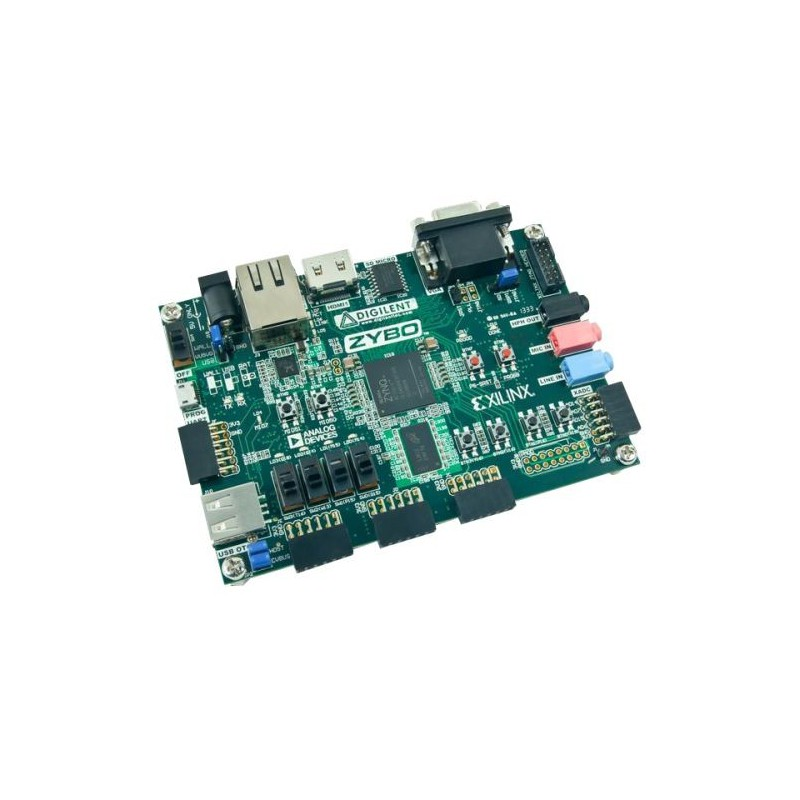
\includegraphics[width=4in]{zybo.jpg}
	%\caption{\label{fig:zybo}Płytka ZYBO Zynq-7000.}
	\captionsource{Płytka ZYBO Zynq-7000.}{\cite{Xi}}
\end{figure}

Zdecydowano, że platformę obliczeniową stanowić będzie płytka ZYBO. Jest to bogato wyposażone narzędzie zawierające układ programowalny z rodziny Xilinx Zynq-7000. Układ ten oparty jest na architekturze Xilinx All Programable System-on-Chip, w której zintegrowany został dwurdzeniowy procesor ARM Cortex-A9 i układ programowalny FPGA z serii Xilinx 7. Zawiera ona m.in. port HDMI potrzebne do odbieranie obrazu z kamery oraz port VGA, który umożliwia nam wysyłanie obrazu do monitora \cite{Xi}. W układzie programowalnym zaimplementowany zostanie tor wizyjny przetwarzający potokowo dane przesyłane z kamery oraz wyznaczający położenie obiektu w danej ramce. Oprócz tego musi on komunikować się ze sterownikiem serwomechanizmów w celu pozycjonowania głowicy w wyznaczonym punkcie oraz z komputerem klasy PC, aby otrzymywać parametry pracy oraz ustawiać początkową pozycję głowicy.

\section{Serwomechanizmy}
\label{sec:serwomechanizmy}

Ruchomą głowicę postanowiono skonstruować wykorzystując serwomechanizmy dostępne na rynku. Przy wyborze brano pod uwagę serwomechanizmy analogowe, serwomechanizmy cyfrowe oraz serwomechanizmy smart.

\subsection{Serwomechanizm analogowy}
Serwomechanizm ten sterowany jest impulsami podawanymi z częstotliwością 50 Hz. Podawanie impulsów z większą częstotliwością może doprowadzić do uszkodzenia urządzenia. W zależności od czasu trwania impulsu serwomechanizm ustawia się w odpowiedniej pozycji i ją utrzymuje. Kontrola położenia odbywa się za pomocą potencjometru sprzężonego z kołem zębatym. Serwomechanizm tego typu nie reagują szybko i nie produkują wystarczającego momentu kiedy zadajemy małe przesunięcie.

\subsection{Serwomechanizm cyfrowy}
Jest on, podobnie jak serwomechanizm analogowy, sterowany impulsami. Podawać można je jednak z maksymalną częstotliwością powyżej 300 Hz. W porównaniu do serwomechanizmu analogowego przyspiesza ono szybciej i produkuje stabilniejszy moment obrotowy. Reagują również lepiej na polecenia małych zmian pozycji. Z drugiej strony  potrzebują one dużo większej mocy. Prąd, który pobierają w trakcie pracy, może sięgać kilku amperów.

\subsection{Serwomechanizm smart}
Główną różnicą pomiędzy serwomechanizmami standardowymi, a smart, jest sposób komunikacji w celu podania wartości zadanej położenia. Zamiast impulsów o różnej szerokości wykorzystuje się komunikację szeregową. Ich obsługa jest więc bardziej skomplikowana. Najpopularniejszymi protokołami są TTL Half-Duplex, TTL Full-Duplex i RS-485. Za pomocą komunikacji tego typu można zmieniać dużo więcej parametrów niż tylko pozycję zadaną. Można zmieniać nastawy regulatora PID, maksymalną prędkość kątową lub maksymalny moment. W przeciwieństwie do serwomechanizmów klasycznych, możemy również odczytywać aktualną pozycję serwomechanizmu. Minusem tych urządzeń jest ich cena oraz dostępność. Są one kilka razy droższe od cyfrowych serwomechanizmów o podobnych parametrach.

\paragraph*{}
Postanowiono użyć dwóch serwomechanizmów cyfrowych PowerHD D-21HV. Są to serwomechanizmy typu standard o dużym momencie obrotowym i wysokiej maksymalnej prędkości obrotowej. Wyposażone jest w łożyska kulkowe oraz tytanowe tryby w celu zwiększenia jego wytrzymałości. Specyfikacja serwomechanizmów:
\begin{itemize}
\item Napięcie zasilania: \(6.0-7.4\) V
\item Zakres ruchu: \(155^\circ\)
\item Masa: \(75\) g
\item Moment: \(21\) kg\(\cdot\)cm dla napięcie \(7.4\) V
\item Prędkość: \(0.12\)s/\(60^\circ\) dla napięcia \(7.4\) V
\end{itemize}
\paragraph*{}
Urządzenia te mogą pobierać impulsowy prąd o wartości nawet powyżej 3 A. Sterowane są za pomocą impulsów podawanych z częstotliwością 333 Hz. Pozycję naturalną zadajemy podając impulsy o czasie trwania \(1500 \mu\)s. Serwa zostały połączone w głowicę za pomocą metalowych uchwytów dedykowanych do łączenia serwomechanizmów typu standard w konfigurację PT.

\section{Sterownik serwomechanizmów}
\label{sec:sterownik}

\begin{figure}[h]
	\centering
	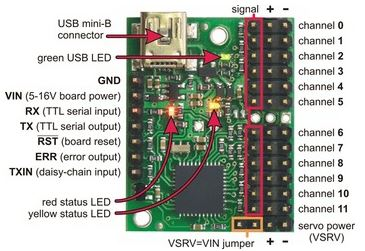
\includegraphics[width=4in]{maestro.jpg}
	\captionsource{Sterownik serwomechanizmów Pololu Mini Maestro.}{\cite{MM}}
\end{figure}

Do sterowania serwomechanizmami postanowiono użyć gotowego sterownika produkowanego przez firmę Pololu. 12-kanałowy sterownik Mini Maestro pozwala na równoczesną obsługę obu serwomechanizmów. Oprócz podawania wartości zadanej w postaci impulsów pozwala on również na zmianę ustawianie maksymalnej prędkości obrotowej i maksymalnego momentu obrotowego. Dzięki temu możemy dużo lepiej kontrolować urządzenia wykonawcze i zapewnić bardziej ciągły ruch głowicy. Komunikujemy się z nim za pośrednictwem interfejsu szeregowego UART z prędkością 115200 bitów na sekundę.

\section{Zasilanie}
\label{sec:zasilanie}
Do zasilania głowicy użyty został zasilacz impulsowy Redox, który na wyjściu daje napięcie 12 V i maksymalny prąd 5 A. Jako, że serwomechanizmy potrzebują napięcia 7.4 V używamy przetwornicy step-down XL4005E1 o regulowanym napięciu wyjściowym. Maksymalny prąd wyjściowy użytej przetwornicy wynosi 5 A. Zdecydowanie wystarczy to do zasilenia użytych serwomechanizmów.

\section{Wskaźnik}
\label{sec:wskaznik}

Postanowiono użyć zwykłego wskaźnika laserowego do wskazywania miejsca, w stronę którego zwrócona jest głowica.
\chapter{Komunikacja}
\label{cha:komunikacja}

Po zbudowaniu stanowiska postanowiono w pierwszej kolejności zaimplementować komunikację między wszystkimi elementami systemu. 
Można ją podzielić na część PC-Zynq oraz Zynq-sterownik serwomechanizmów "Maestro".
%TODO Maestro - niesjane... -zrobione.

\section{PC-Zynq}
\label{sec:pc-zynq}
Postanowiono wykorzystać UART. 
Argumentem przemawiającym za tym rozwiązaniem był fakt wyprowadzenia dwóch pinów MIO (48 i 49) procesora karty ZYBO do złącza mikro USB typu B. 
Piny te podłączone zostały do jednego z układów procesora odpowiedzialnych za komunikację szeregową - UART1. 
Złącze USB służy również do programowania układu przez JTAG.
Dzięki temu używa się jednego przewodu do programowania układu oraz do komunikacji z nim. 
Po podłączeniu przewodu oraz włączeniu ZYBO w komputerze pojawia się dodatkowy port COM. 
Przez ten port można wymieniać dane z platformą obliczeniową. Do wysyłania komunikatów na PC wykorzystano program \textit{Realterm}. 
Dzięki temu nie było konieczności pisania dodatkowego oprogramowania. Okno programu \textit{Realterm} zostało przedstawione na rysunku \ref{fig:realterm}.

\begin{figure}[h]
	\centering
	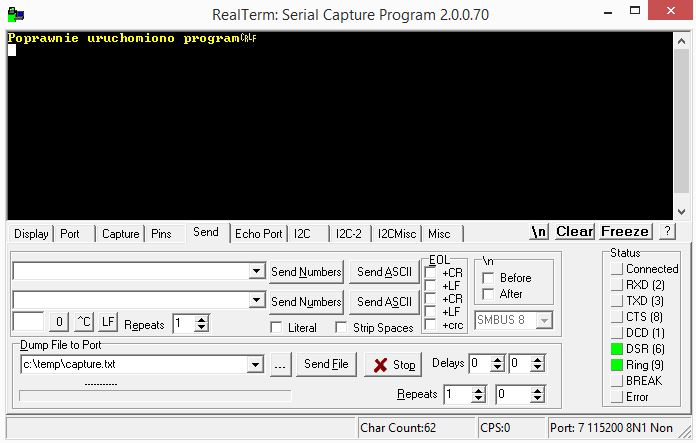
\includegraphics[width=4in]{realterm.jpg}
	\caption{Okno programu Realterm z komunikatem o poprawnym uruchomieniu programu.}
	\label{fig:realterm}
\end{figure}

\paragraph*{}
Rozmiar jednej komendy wysyłanej do układu Zynq wynosi 5 bajtów.
Pierwszy informuje o typie rozkazu, a 4 kolejne są danymi do tego rozkazu.
Każdy kolejny odebrany bajt umieszczany jest w buforze o rozmiarze 5 bajtów.
Włączone zostało przerwanie od pełnego bufora.
Po wysłaniu komendy z PC w procesorze układu Zynq uruchamiane jest przerwanie, w którym wysłany zostaje odpowiedni rozkaz do sterownika serwomechanizmów lub ustawiana jest zmienna informująca o pracy w trybie autonomicznym, podczas którego kamera ustawiana jest tak, by obiekt znajdował się w centrum kadru.
%TODO niejasne, bo wczesniej tryb autonomiczny sie nie pojawił. -zrobione.
Zaimplementowano obsługę następujących komend w Zynq:
\begin{itemize}
\item Zmiana pozycji serwomechanizmów: 0x00 0xHH 0xLL 0xHH 0xLL.
\item Zmiana maksymalnej prędkości serwomechanizmów: 0x01 0xHH 0xLL 0xHH 0xLL.
\item Zmiana maksymalnego momentu serwomechanizmów: 0x02 0xHH 0xLL 0xHH 0xLL.
\item Odczyt aktualnej wartości zadanej ze sterownika: 0x03 0x-- 0x-- 0x-- 0x--.
\item Rozpoczęcie pracy autonomicznej (śledzenia): 0x04 0x-- 0x-- 0x-- 0x--.
\end{itemize}
\paragraph*{}
W pierwszych trzech rozkazach pierwsze dwa bajty danych są parametrami dla serwomechanizmu odpowiedzialnego za obrót, a kolejne dwa są parametrami dla serwomechanizmu odpowiedzialnego za nachylenie. 
Myślniki w kolejnych komendach oznaczają, że wysłane bajty danych nie są istotne (komendy te nie potrzebują danych).

\section{Zynq-Maestro}
\label{sec:zynq-maestro}

% Tutaj wstaw zdjęcie połączonego układu ZYBO-Maestro.

Komunikacja przez UART została narzucona, gdyż jest to jedyny protokół komunikacyjny w Maestro. 
Połączone zostały odpowiednie piny (MIO 14,15) złącza MIO PMOD karty ZYBO do pinów Maestro odpowiadających za komunikację szeregową.
Następnie do użytych pinów MIO podłączono wyjścia innego układu procesora odpowiadającego za komunikację szeregową - UART0.
W dokumentacji Maestro wyszukano listę komend i zaimplementowano wysyłanie potrzebnych w układzie Zynq \cite{MM}. Są to następujące komendy:
\begin{itemize}
\item Zmiana pozycji serwomechanizmów: 0x9F 0x02 0x0A 0xLL 0xHH 0xLL 0xHH.
\item Zmiana maksymalnej prędkości serwomechanizmów: 0x87 0x0A/0x0B 0xLL 0xHH.
\item Zmiana maksymalnego momentu serwomechanizmów: 0x89 0x0A/0x0B 0xLL 0xHH.
\item Odczyt pozycji ze sterownika: 0x90 0x0A/0x0B.
\end{itemize}
W powyższych komendach A oznacza obrót, a B nachylenie (są to numery kanałów sterownika zapisane szesnastkowo).

\section{Testy komunikacji}
\label{testy_komunikacji}
Komunikacja była testowana na układzie złożonym z:
\begin{itemize}
\item Komputera klasy PC.
\item Karty ewaluacyjnej ZYBO.
\item Komputera Raspberry Pi 2 Model B.
\end{itemize}
Karta ZYBO połączona wraz z połączonym komputerem Raspberry Pi 2 B zostały przedstawione na rysunku \ref{fig:raspberry}.

\begin{figure}[h]
	\centering
	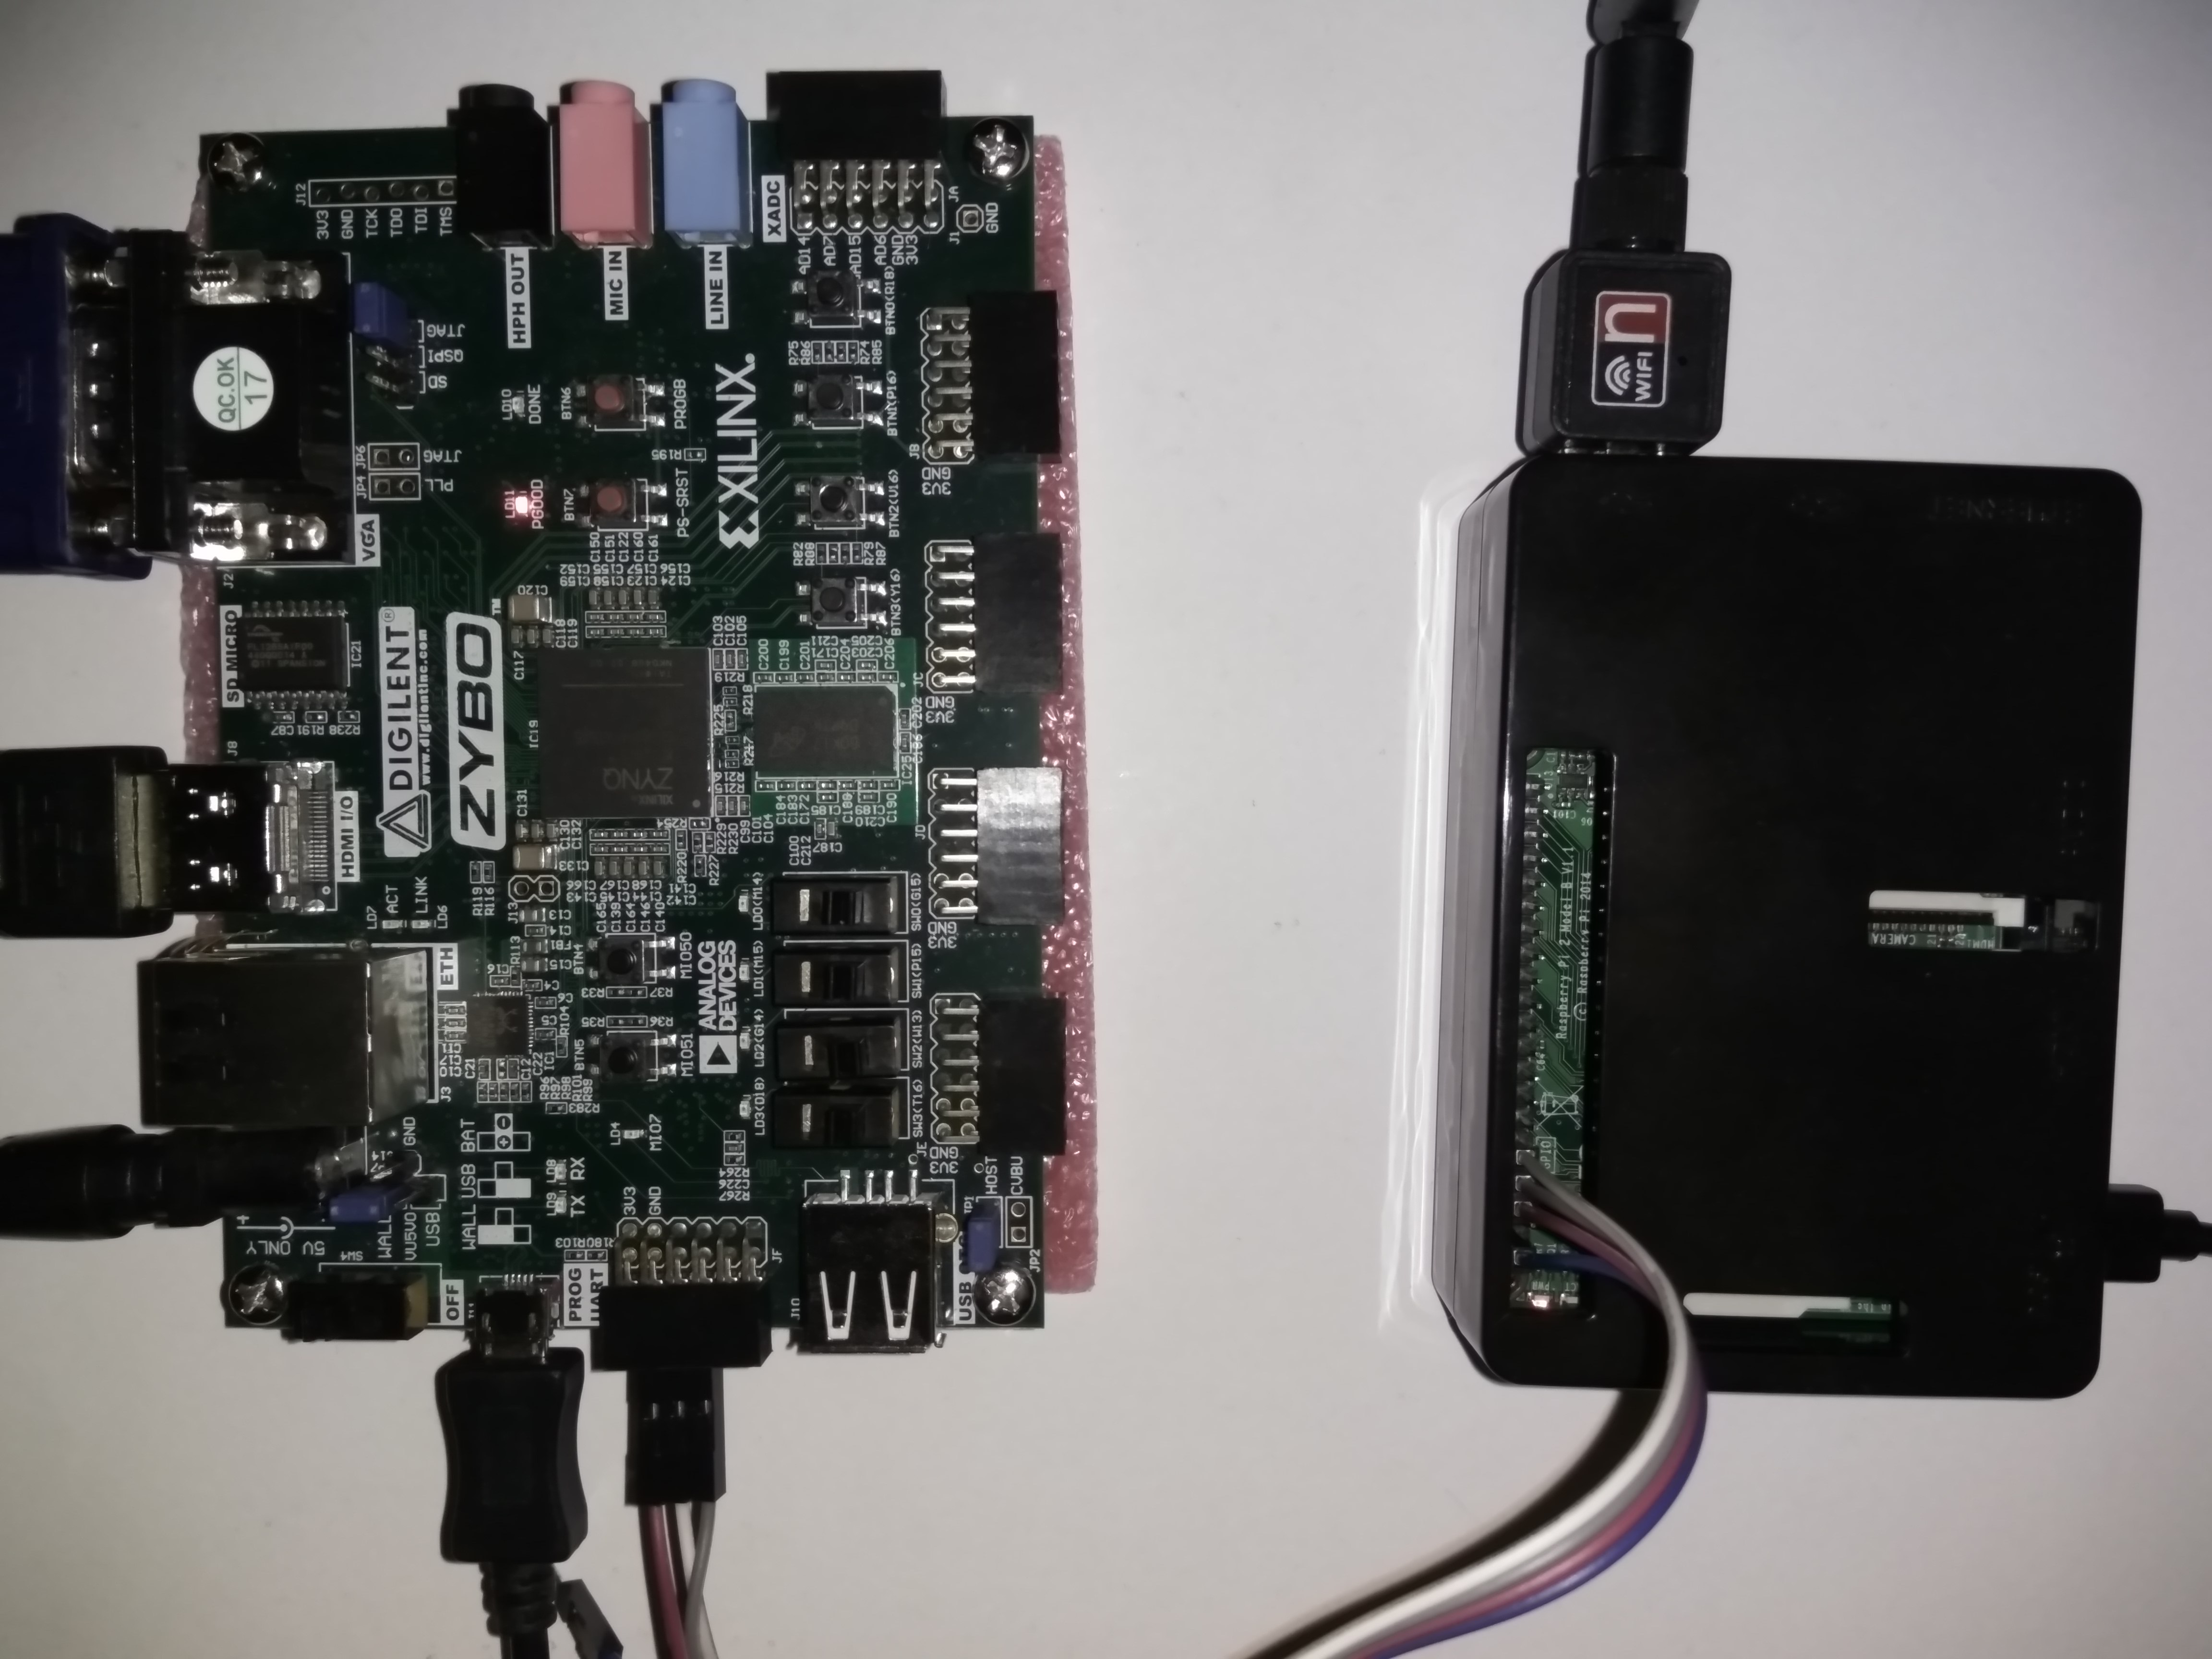
\includegraphics[width=4in]{raspberry.jpg}
	\caption{Karta ewaluacyjna ZYBO i komputer Raspberry pi 2 B użyty do testów.}
	\label{fig:raspberry}
\end{figure}

\paragraph*{}
W układzie tym Raspberry zastępowało sterownik serwomechanizmów.
Zamiana ta została wykonana, by mieć możliwość sprawdzania poprawności danych odbieranych z Zynq.
W trakcie testów okazało się, że pierwszy bajt wysyłany do ZYBO jest wpisywany do bufora i wskaźnik jest przesuwany, lecz w kontrolerze przerwań nie jest zwiększany licznik liczby bajtów w buforze.
W efekcie przerwanie od pełnego bufora danych przychodzących było wywoływane o 1 bajt za późno (po otrzymaniu pierwszego bajtu nowej komendy).
Naprawiono to poprzez dodatkowy test w trakcie inicjalizacji komunikacji szeregowej.
Polegał on na włączeniu trybu \textit{loopback}, wysłaniu i odebraniu kilku bajtów danych, a następnie zresetowaniu bufora. W trybie \textit{loopback} dane wysyłane przez UART są wysyłane na jego wejście.
W ten sposób można sprawdzać zgodność danych.
Oprócz tego sprawdzono, czy wysłanie komendy z PC do Zynq skutkuje wysłaniem poprawnej komendy z Zynq do Maestro.
Po naprawieniu opisanego problemu i ponownym przeprowadzeniu testów stwierdzono, że komunikacja działa poprawnie.
\chapter{Tor wizyjny}
\label{cha:torwizyjny}

Kolejnym krokiem realizacji projektu była implementacja podstawowych zadań przetwarzania obrazu w logice rekonfigurowalnej układu heterogenicznego. 
Rozpoczęto od stworzenia podstawowego toru wizyjnego pobierającego obraz z wejścia HDMI i~wysyłającego go bez zmian na wyjście VGA. 
Następnie stworzono moduły pozwalające na realizację algorytmu śledzenia przez detekcję.

\section{Podstawowe przesyłanie obrazu}
\label{sec:podstawoweprzesylanieobrazu}
Tor wizyjny nie wykonujący żadnych zmian w obrazie pozwoli nam na określenie czy dane są poprawnie odbierane z kamery i poprawnie wysyłane do monitora. 
Stanowić on będzie również bazę dla dowolnego innego realizowanego algorytmu przetwarzania obrazu. 
Konieczna jest więc pewność, że działa poprawnie. 
Musi on realizować następujące zadania:
\begin{enumerate}
\item Odbieranie danych ze złącza HDMI/DVI.
\item Dekodowanie danych odebranych ze złącza HDMI/DVI do postaci przestrzeni barw RGB i sygnałów synchronizacyjnych.
%TODO nie podoba mi się to stwierdzenie. one po HDMI są przesyłane w RGB więc to nie ma konwersji. Jest dekodowanie do postaci RGB i sychronizacji -zrobione.
\item Kodowanie danych z przestrzeni barw RGB i sygnałów synchronizacyjnych do VGA.
%TODO jw. -zrobione.
\item Wysłanie danych do złącza VGA.
\end{enumerate}
Zadania te są realizowane przez moduły dostarczane przez firmę \textit{Digilent}, producenta platformy obliczeniowej.
Moduły połączone zostały w schemacie blokowym programu \textit{Vivado}, co pokazano na rysunku \ref{fig:tor_wizyjny}.
%TODO co to znaczy, że za pomocą diagramu ??? styl -zrobione.
Schemat blokowy, w porównaniu do pliku języka Verilog, zwiększa przejrzystość połączeń między modułami oraz zmniejsza ryzyko błędu np. w nazwie portu.
%TODO Odniesienie  w txt do rysunku (do każdego mu być !!!) -zrobione.
%TODO To dla odmiany mogłoby być większe.... na całą szerokość strony. -zrobione.
%TODO Przydałoby się też omówienie posczególych modułów. -zrobione.

\paragraph*{}
Do stworzenia schematu widocznego na rysunku \ref{fig:tor_wizyjny} wykorzystano następujące moduły:\begin{itemize}
\item \textit{Clocking Wizard} - Generacja sygnału zegarowego o częstotliwości \(200\)MHz.
\item \textit{DVI to RGB Video Decoder} - Dekodowanie danych odebranych ze złącza HDMI/DVI do postaci przestrzeni barw RGB i sygnałów synchronizacyjnych.
\item \textit{RGB unpack} - Zamiana 24-elementowego wektora przestrzeni barw do osobnych, 8-elementowych wektorów (R, G, B).
\item \textit{RGB pack} - Zamiana trzech 8-elementowych wektorów (R, G, B) do jednego 24-elementowego wektora przestrzeni barw.
\item \textit{RGB to VGA output} - Kodowanie danych z przestrzeni barw RGB i sygnałów synchronizacyjnych do VGA.
\end{itemize}

\begin{figure}[h]
	\centering
	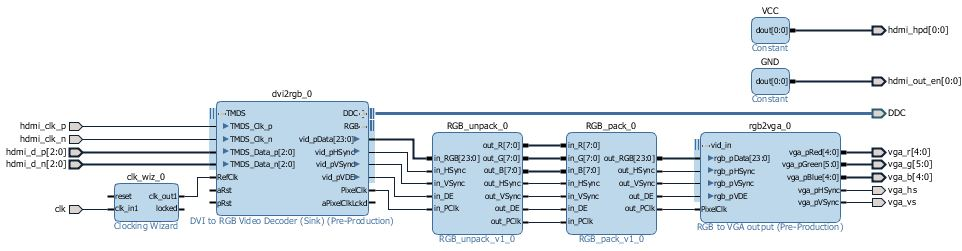
\includegraphics[width=6in]{Tor_wizyjny.jpg}
	\caption{Podstawowy tor wizyjny.}
	\label{fig:tor_wizyjny}
\end{figure}

\paragraph*{}
Testy rozpoczęto od podłączenie wyjścia HDMI laptopa do wejścia HDMI karty ZYBO oraz podłączenia monitora do wyjścia VGA ZYBO. W tak połączonym układzie obraz był wyświetlany poprawnie. Następnie źródło obrazu zamieniono na docelową kamerę. 
W tym przypadku obraz nie został wyświetlony na ekranie monitora. 
W celu znalezienia i naprawy problemu postanowiono w torze wizyjnym włączyć opcję \textit{debug} dla części węzłów. 
Dzięki temu można podglądać sygnały już w działającym układzie.
Ustalono, że problem występuje w module odbierającym dane z wejścia HDMI - \textit{dvi2rgb}. 
Problem udało się naprawić aktualizując go z wersji 1.2 do wersji 1.6, wyłączając bufor dla sygnału zegarowego (opcja \textit{Add BUFG to PixelClk}), włączając opcję \textit{Enable DDC ROM}, zmieniając zakres zegara taktującego TMDS do \(<120\) MHz oraz preferowaną rozdzielczość przetwarzanego obrazu na 1280x720.
%TODO A może Pan napisać szczegóły (do jakich parametrów) -zrobione.

\section{Śledzenie przez detekcję}
\label{sec:sledzenieprzezdetekcje}

Śledzenie przez detekcję zostało zrealizowane na podstawie koloru śledzonego obiektu. 
Jako parametr modułu detekcji podawany jest zakres kolorów w przestrzeni barw RGB, które mają być traktowane jako należące do obiektu. 
Pikselowi, którego kolor mieści się w podanym zakresie przypisywana jest wartość 1, a pozostałym 0. 
Pod nadaniu wartości wszystkim pikselom kadru obliczany jest środek ciężkości obrazu. 
W~ten sposób wyznaczono środek śledzonego obiektu. 
Punkt ten zaznaczany jest na obrazie wyjściowym za pomocą dwóch czerwonych linii - poziomej i pionowej. 
Podczas testów wykrywany był następujący zakres przestrzeni barw RGB, odpowiadający kolorowi zielonemu:
\begin{equation}
R \in [0,30]
\end{equation}
\begin{equation}
G \in [40,255]
\end{equation}
\begin{equation}
B \in [0,30]
\end{equation}
Przykładowy wynik działania opisanego modułu przedstawiono na rysunku \ref{fig:detekcja}.

\begin{figure}[H]
	\centering
	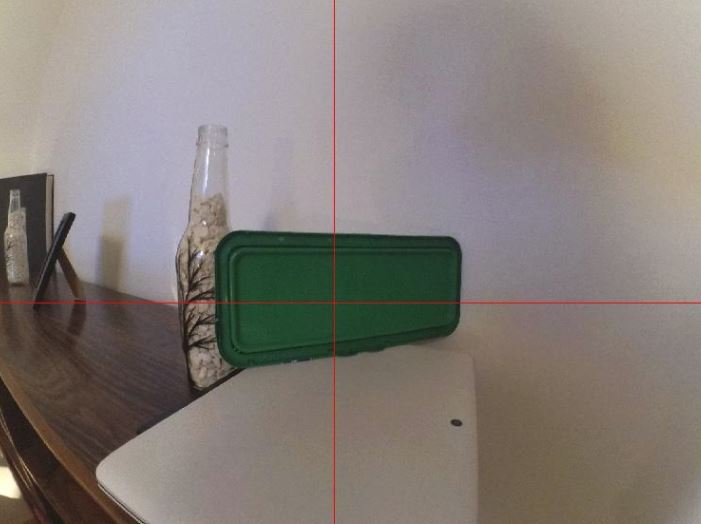
\includegraphics[width=4in]{detekcja.jpg}
	\caption{Przykładowy wynik działania algorytmu.}
	\label{fig:detekcja}
\end{figure}
%TODO odnośnik. No i jakiś mało sugestywny przykład ? to jest w paint ? czy jak ? Nie da się rzeczywistego zdjęcia dać. -zrobiene.

Testy były wykonywane zarówno dla obrazu z komputera PC jak i kamery. 
Należy zwrócić uwagę na niską efektywność tej metody dla obrazu z kamery. 
Spowodowane jest to szumami oraz bardzo dużą zależnością rozpoznanego koloru od natężenia i rodzaju oświetlenia.

\section{Komunikacja PL-PS}
\label{komunikacjapl-ps}

Połączono wykonany w tym rozdziale tor wizyjny i wyznaczanie środka ciężkości z komunikacją zaimplementowaną w rozdziale \ref{cha:komunikacja}.
Dzięki temu zintegrowano stworzone do tej pory moduły w funkcjonalną całość.
W tym celu należało zastosować komunikację pomiędzy procesorem ARM, a FPGA.
%TODO Styl.... trzeba napisać po co - Czy tak lepiej?
Odbywa się ona z użyciem modułu \textit{AXI Lite}.
Do procesora wysyłane są współrzędne wyznaczonego środka ciężkości śledzonego obiektu. 
Kiedy dane są gotowe do odczytu, sygnał oznaczający wysłanie danych do procesora zmienia wartość logiczna z \(0\) na \(1\).
Od narastającego zbocza tego sygnału zgłaszane jest przerwanie, w którym aktualizowana jest zmienna odpowiedzialna za położenie celu, czyli wartości zadane serwomechanizmów. 
W procesorze odebrane współrzędne przeliczone zostają na uchyby regulacji kątów na podstawie rozdzielczości obrazu i kątów nagrywania kamery. 
Założono, że odległość pikseli od środka obrazu jest proporcjonalna do kąta.
Założenie to nie jest słuszne w ogólności, ale jest prawdziwe dla małych wartości odchylenia.
Wyznaczenie dokładnej wielkości wymagałoby użycia Lookup table (tablicy przyporządkowującej każdemu pikselowi wartość kąta) lub wyznaczania funkcji matematycznej wykonującą powyższą funkcję.
%TODO dziwne zdanie...a to nie jest tak, że dla małych kątów...
%MK: Nie wiem czy teraz lepiej. Starałem się to inaczej opisać.
%TODO no ale chyba tylko dla dwóch liczb


%TODO Rozważyłbym jednak śledzenie przez detekcję przenieść przed meanshift, zeby algorytmy śledzące były jeden obok drugiego.
%MK: Pomyślę, co trzebaby wtedy zmienić, żeby to było ok.

%TODO Może jakieś zdjęcie jak to działa, a to było już z serwami robione?
%MK: Kiedy to robiłem to jeszcze nie z serwami, ale później testowałem to z nimi i działało. Ciężko na zdjęciu pokazać, jak się poruszają serwa za obiektem. A samo zdjęcie ze środka ciężkości już jest wyżej. Czy ma Pan jakiś pomysł jak w pracy pokazać, że serwa się poruszają za obiektem? Do prezentacji na pewno filmiki muszę nagrać.
\chapter{Regulator}
\label{cha:regulator}

W zaprojektowanym układzie kamera pełni rolę sensora uchybu regulacji. Układ nie ma możliwości mierzenia pozycji serwomechanizmów. Aby poprawnie pozycjonować musimy więc zaimplementować regulator, którego wyjściem będzie wartość zadana serwomechanizmów.

\section{Model układu}
\label{sec:modelukladu}

Aby mieć możliwość testowania regulatora bez konieczności każdorazowej zmiany kodu źródłowego oraz ryzyka uszkodzenia układu postanowiono wyznaczyć model układu, a następnie przeprowadzić badania symulacyjne w programach \textit{MATLAB} i \textit{Simulink}. Na podstawie modelu możemy również dobrać parametry regulatora, które zapewnią asymptotyczną stabilność oraz szybkie pozycjonowanie układu. Rozpoczęto od wyznaczenia transmitancji serwomechanizmów. Wiadomo, że w serwomechanizmie jest regulator proporcjonalny.

\begin{figure}[h]
	\centering
	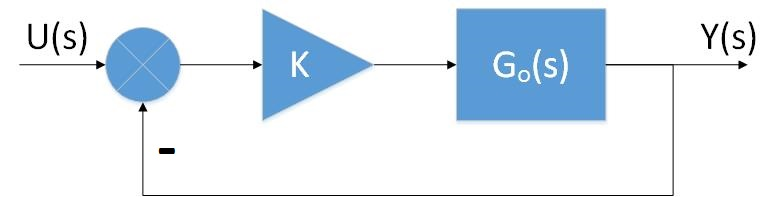
\includegraphics[width=4in]{servo.jpg}
	\captionsource{Schemat blokowy serwomechanizmu.}{Własne}
\end{figure}

\(G_o(s)\) jest transmitancją silnika prądu stałego, gdy wejściem jest napięcie, a położenie kątowe wału silnika:
\begin{equation}
G_o(s)=\frac{1}{s(Ts+1)}
\end{equation}
\(K\) jest wzmocnieniem regulatora proporcjonalnego.\newline
Transmitancja zastępcza powyższego układu wynosi:
\begin{equation}
\label{eq:servo}
G_s(s)=\frac{K}{Ts^2+s+K}
\end{equation}
Ze względu na brak enkoderów w układzie, nie można przeprowadzić identyfikacji parametrów serwomechanizmów. Na podstawie obserwacji wiadomo, że w wzmocnienie regulatora jest dobrane tak, by silnik nie oscylował wokół wartości zadanej. Powinno być ono wzmocnieniem krytycznym dla danego silnika. Aby wzmocnienie \(K\) było krytyczne, musi być ono równe:
\begin{equation}
\label{eq:kryt}
K=\frac{1}{4T}
\end{equation}
Podstawiając powyższy wzór do równania \ref{eq:servo} otrzymuje się:
\begin{equation}
G_s(s)=\frac{1}{4T^2s^2+4Ts+1}
\end{equation}
Wartość stałej czasowej jest przyjęta na podstawie odpowiedzi skokowej serwomechanizmu.
\begin{equation}
T=0.05
\end{equation}
Następnie wykonano schemat blokowy kompletnego układu (z kamerą i implementowanym regulatorem).

\begin{figure}[h]
	\centering
	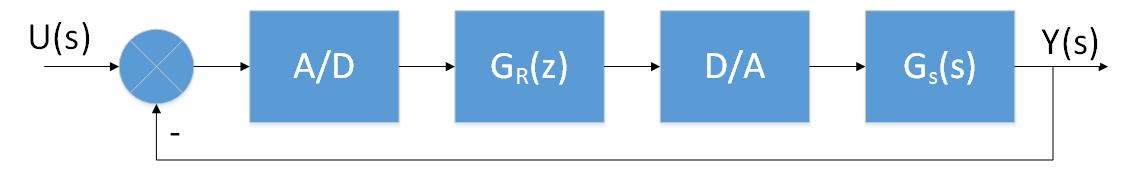
\includegraphics[width=4in]{uklad.jpg}
	\captionsource{Schemat blokowy kompletnego układu.}{Własne}
\end{figure}

\(G_R(z)\) jest transmitancją projektowanego regulatora dyskretnego.
\paragraph*{}
Rolę przetwornika A/D pełni w układzie kamera, a przetwornika D/A sterownik serwomechanizmów. Schemat ten można przedstawić w następującej, równoważnej postaci.

\begin{figure}[h]
	\centering
	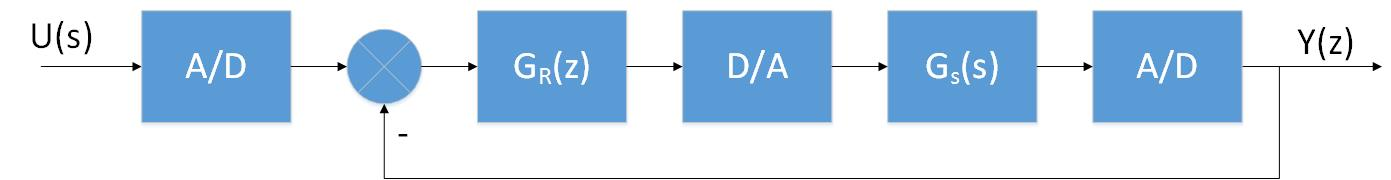
\includegraphics[width=4in]{uklad_digital.jpg}
	\captionsource{Równoważny schemat kompletnego układu.}{Własne}
\end{figure}

Transmitancję opisaną równaniem \ref{eq:servo} można zapisać za pomocą równań stanu:
\begin{equation}
\dot{x}=Ax+Bu
\end{equation}
\begin{equation}
y=Cx
\end{equation}
\begin{equation}
A=
	\begin{bmatrix}
	0 & 1 \\
	-\frac{K}{T} & -\frac{1}{T}
	\end{bmatrix}
\end{equation}
\begin{equation}
B=
	\begin{bmatrix}
	0 \\
	1
	\end{bmatrix}
\end{equation}
\begin{equation}
C=
	\begin{bmatrix}
	\frac{K}{T} & 0
	\end{bmatrix}
\end{equation}
Wzmocnienie krytyczne regulatora w serwomechanizmach dobrane jest dla silników bez obciążenia. Jeśli silnik zostaje obciążony, to zwiększa się jego stała czasowa. Wzmocnienie więc również powinno być zmienione. Wziąć należy jednak pod uwagę, że masa użytej kamery jest mała w porównaniu do maksymalnej masy obciążenia tych urządzeń. Z tego względu można przyjąć, że stała czasowa nie zmienia się, a wzmocnienie nadal jest krytyczne. Nadal zachodzi więc równanie \ref{eq:kryt}. Podstawiono je do powyższych macierzy.
\begin{equation}
A=
	\begin{bmatrix}
	0 & 1 \\
	-\frac{1}{4T^2} & -\frac{1}{T}
	\end{bmatrix}
\end{equation}
\begin{equation}
B=
	\begin{bmatrix}
	0 \\
	1
	\end{bmatrix}
\end{equation}
\begin{equation}
C=
	\begin{bmatrix}
	\frac{1}{4T^2} & 0
	\end{bmatrix}
\end{equation}
Obiekt ten można razem z przetwornikiem A/D i przetwornikiem D/A pierwszego rzędu przedstawić można jako jeden równoważny obiekt dyskretny. Wyznaczono następnie równania stanu tego obiektu \cite{TS}.
\begin{equation}
\label{eq:A^+}
A^+=e^{hA}
\end{equation}
\begin{equation}
\label{eq:B^+}
B^+=\int\limits_{0}^{h}e^{tA}Bdt
\end{equation}
\begin{equation}
C^+=C
\end{equation}
\(h\) oznacza okres próbkowania dyskretnej części układu.
\begin{equation}
h=\frac{1}{60}
\end{equation}
Obliczenia rozpoczęto od wyliczenia macierzy \(e^{tA}\).
\begin{equation}
e^{tA}=\mathcal{L}^{-1}[(sI-A)^{-1}]
\end{equation}
\begin{equation}
e^{tA}=\mathcal{L}^{-1}
	\begin{bmatrix}
	\frac{s+\frac{1}{T}}{(s+\frac{1}{2T})^2} & \frac{1}{(s+\frac{1}{2T})^2} \\
	\frac{-\frac{1}{4T^2}}{(s+\frac{1}{2T})^2} &  \frac{s}{(s+\frac{1}{2T})^2}
	\end{bmatrix}
\end{equation}
\begin{equation}
\label{eq:e^tA}
e^{tA}=
	\begin{bmatrix}
	(1+\frac{t}{2T})e^{-\frac{t}{2T}} & te^{-\frac{t}{2T}} \\
	-\frac{t}{4T^2}e^{-\frac{t}{2T}} & (1-\frac{t}{2T})e^{-\frac{t}{2T}}
	\end{bmatrix}
\end{equation}
Podstawiono \ref{eq:e^tA} do \ref{eq:A^+} i \ref{eq:B^+}.
\begin{equation}
A^+=
	\begin{bmatrix}
	(1+\frac{h}{2T})e^{-\frac{h}{2T}} & he^{-\frac{h}{2T}} \\
	-\frac{h}{4T^2}e^{-\frac{h}{2T}} & (1-\frac{h}{2T})e^{-\frac{h}{2T}}
	\end{bmatrix}
\end{equation}
\begin{equation}
B^+=\int\limits_{0}^{h}
	\begin{bmatrix}
	te^{-\frac{t}{2T}} \\
	(1-\frac{t}{2T})e^{-\frac{t}{2T}}
	\end{bmatrix}
	dt
\end{equation}
\begin{equation}
\int te^{-\frac{t}{2T}}=-2Tte^{-\frac{t}{2T}}+2T\int e^{-\frac{t}{2T}}dt
\end{equation}
\begin{equation}
\int te^{-\frac{t}{2T}}=-2Tte^{-\frac{t}{2T}}-4T^2e^{-\frac{t}{2T}}
\end{equation}
\begin{equation}
B^+=
	\begin{bmatrix}
	-2T(h+2T)e^{-\frac{h}{2T}}+4T^2 \\
	he^{-\frac{h}{2T}}
	\end{bmatrix}
\end{equation}
\begin{equation}
C^+=
	\begin{bmatrix}
	\frac{1}{4T^2} & 0
	\end{bmatrix}
\end{equation}
Aby sprawdzić poprawność przeprowadzonych obliczeń postanowiono porównać odpowiedzi skokowe układu ciągłego i dyskretnego. Do tego celu zostało wykorzystane środowisko \textit{MATLAB}.

\begin{figure}[h]
	\centering
	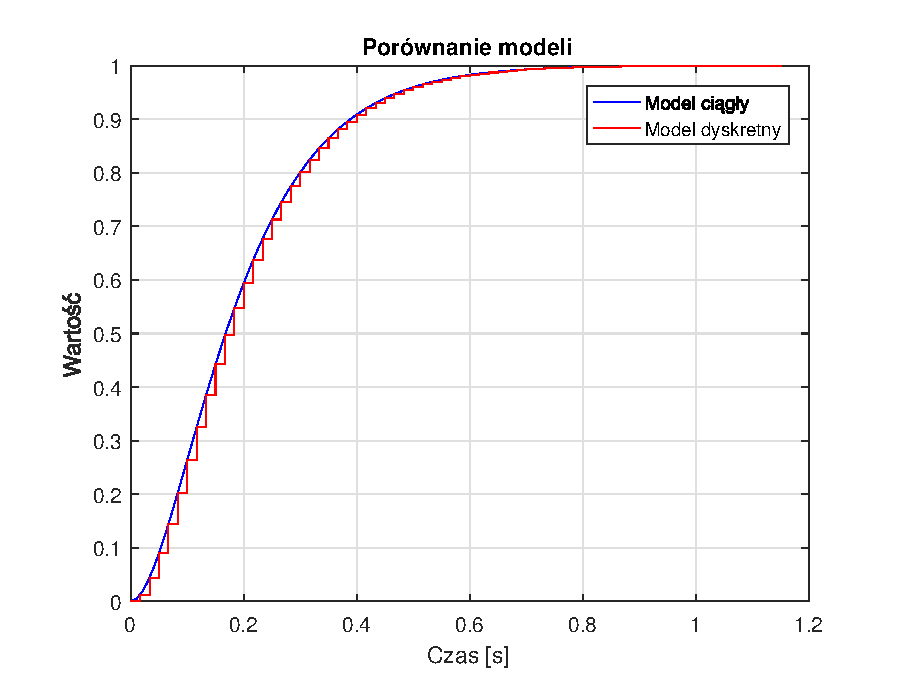
\includegraphics[width=4in]{comp.eps}
	\captionsource{Porównanie modelu ciągłego oraz odpowiadającego mu dyskretnego.}{Własne}
\end{figure}

Na podstawie powyższego wykresu można wnioskować, że wyliczony model jest poprawny. Należy jednak zwrócić uwagę na fakt, że w rzeczywistym układzie występują występują dodatkowo opóźnienia, które nie zostały uwzględnione w modelu. Z tego względu model nie będzie idealnie odpowiadał działaniu rzeczywistego układu.

\paragraph*{}
Kompletny model układu postanowiono zaimplementować w programie \textit{Simulink}. Uwzględnia on:
\begin{itemize}
\item Nasycenie wartości zadanej serwomechanizmów
\item Przeliczanie współrzędnych śledzonego obiektu na kąty
\item Obliczanie szerokości impulsów wysyłanych do serwomechanizmu
\item Kwantyzację liczby pikseli i szerokości impulsów
\end{itemize}

\begin{figure}[h]
	\centering
	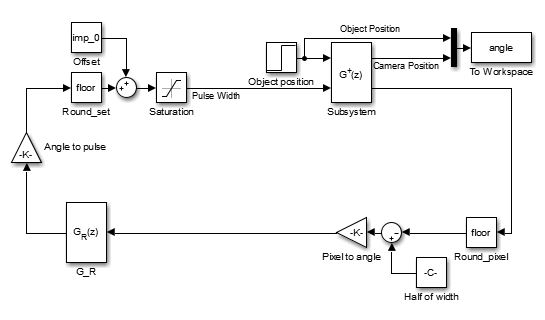
\includegraphics[width=4in]{Simulink.jpg}
	\captionsource{Model układu zrealizowany w programie \textit{Simulink}.}{Własne}
\end{figure}

\section{Projekt regulatora}
\label{sec:projektregulatora}

W układzie nie ma czujnika pozycji serwomechanizmów, więc algorytm regulacji musi bazować na wyjściu z poprzedniej iteracji. Algorytmem, który działa w ten sposób jest prędkościowy (przyrostowy) regulator PID. Zaimplementowany regulator ma następującą postać:
\begin{equation}
u(k)-u(k-1)=P \cdot (e(k)-e(k-1))+I \cdot e(k)+D \cdot (e(k)-2e(k-1)+e(k-2))
\end{equation}
Został on zrealizowany w programie \textit{Simulink}.

\begin{figure}[h]
	\centering
	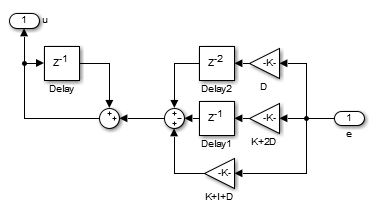
\includegraphics[width=4in]{Przyrostowy.jpg}
	\captionsource{Realizacja przyrostowego regulatora PID.}{Własne}
\end{figure}

Na podstawie odpowiedzi modelu dobrano następujące wartości parametrów:
\begin{equation}
P=1
\end{equation}
\begin{equation}
I=0.1
\end{equation}
\begin{equation}
D=0.2
\end{equation}

\begin{figure}[H]
	\centering
	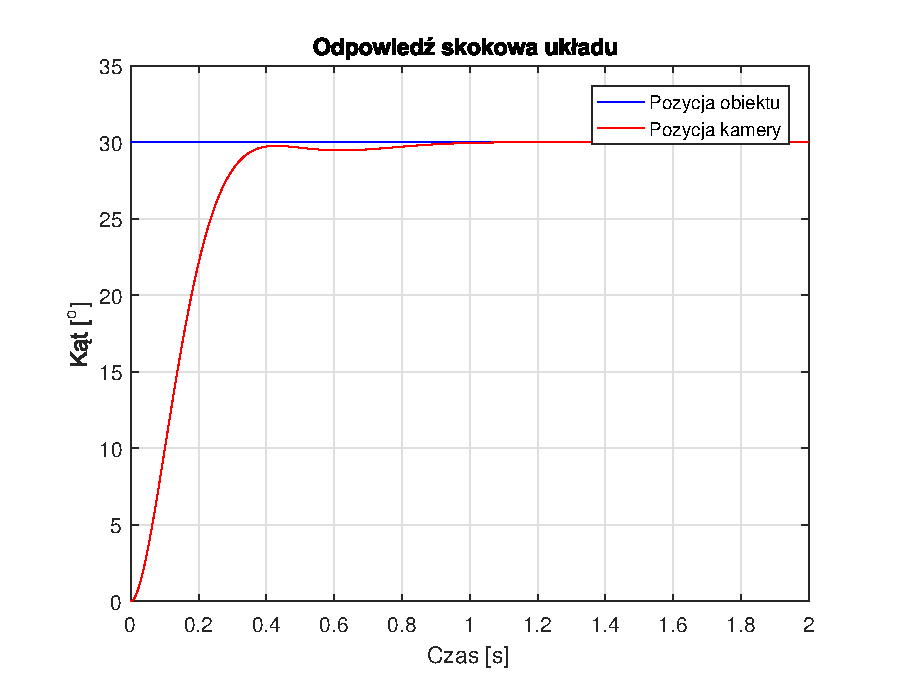
\includegraphics[width=3.4in]{sim_step.eps}
	\captionsource{Odpowiedź skokowa układu z dobranym regulatorem.}{Własne}
\label{fig:sim_step}
\end{figure}

\begin{figure}[H]
	\centering
	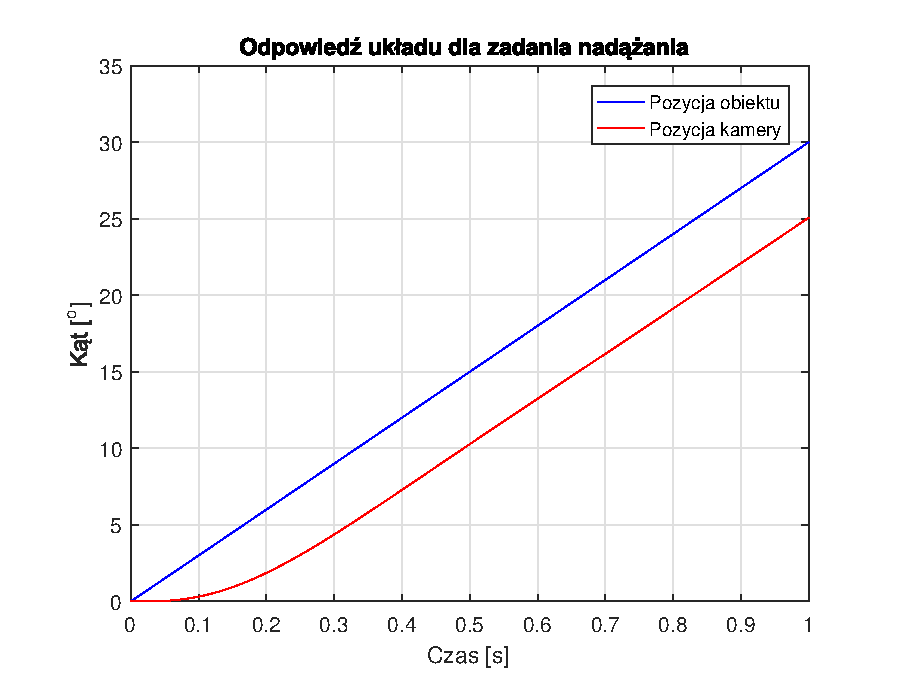
\includegraphics[width=3.4in]{sim_ramp.eps}
	\captionsource{Odpowiedź układu dla zadania nadążania.}{Własne}
\label{fig:sim_ramp}
\end{figure}

Na wykresie \ref{fig:sim_step} widać, że układ szybko reaguje na skokowe zmiany pozycji śledzonego obiektu. Z kolei na wykresie \ref{fig:sim_ramp} zauważyć można, że obecny jest uchyb ustalony dla zadania nadążania. Aby się go pozbyć konieczne byłoby zastosowanie w układzie dodatkowego członu całkującego szeregowo użytym regulatorze, co zwiększyłoby rząd stosowanego rozwiązania. Użyte parametry mogą zostać skorygowane w rzeczywistym układzie w zależności od rezultatów i wpływu pominiętych efektów.
\chapter{Tor wizyjny z algorytmem Mean-shift}
\label{cha:torwizyjnyzalgorytmemmeanshift}

Przekształcono tor wizyjny zbudowany w rozdziale \ref{cha:torwizyjny} tak, by źródłem położenia obiektu był gotowy algorytm Mean-shift, który został opisane w sekcji \ref{sec:meanshift}. Rozpoczęto od przystosowania otrzymanego modułu tak, by bardziej nadawał się do celów projektu. Najpierw zmieniono sposób podawania rozmiaru okna oraz początkowego jego położenia z inicjalizacji rejestrów odpowiednimi wartościami na parametry modułu. Dzięki temu podczas testów nie trzeba generować ponownie modułu w celu zmiany powyższych parametrów. Oprócz tego dodano sygnał wyjściowy informujący o wyznaczeniu nowego położenia środka obiektu. Używany on jest do wysyłania współrzędnych środka do procesora oraz do zgłoszenia przerwania w procesorze.

\paragraph*{}
Użyty algorytm Mean-shift wylicza wartości prawdopodobieństwa dla pikseli na podstawie histogramu ich otoczenia i histogramu początkowej ramki. Działa on na obrazie w skali szarości. Jego działanie może być więc w dużej mierze zależne od użytej metody konwersji przestrzeni barw RGB. Postanowiono najpierw użyć wartości składowej Y z przestrzeni barw YUV. Obliczana jest ona następująco:
\begin{equation}
\label{eq:grayscale}
Y=0.299 \cdot R+0.587 \cdot G+0.114 \cdot B
\end{equation}
Bierze się w ten sposób pod uwagę, że oko ludzki jest najbardziej wyczulone na kolor zielony, a najmniej na kolor niebieski. Do wykonania powyższej konwersji zostały użyte 3 moduły mnożarki w układzie FPGA.
Oprócz wartości piksela i sygnałów synchronizacyjnych na wejście podawany jest również sygnał ustawienia histogramu obiektu. Zapisywany jest wtedy histogram obiektu aktualnie znajdującego się w oknie. Sygnał ten został podłączony do przełącznika znajdującego się na płytce ZYBO. Wyjście modułu realizującego śledzenie zostało wyprowadzone do modułu, który na obrazie wyjściowym zaznacza aktualne okno.

\paragraph*{}
Najpierw sprawdzono działanie zaimplementowanego systemu podając na wejście HDMI obraz z komputera PC. Było nim czarne koło na białym tle. Przesuwano koło i sprawdzano, czy zaznaczone okno będzie się przesuwać razem z nim. Na podstawie wyników stwierdzono, że algorytm działa, lecz gubi obiekt, kiedy ten porusza się zbyt szybko, lub wykona jakiś gwałtowny ruch. Może to być bardzo problematyczne w trakcie śledzenia rzeczywistego obiektu. Dla obrazu z kamery nie będzie również tak dobrze rozróżniony obiekt od tła. Można się więc domyślać, że algorytm ten dużo gorzej będzie działać w rzeczywistym układzie.

\paragraph*{}
Następnie na wejście HDMI podano obraz z kamery używanej w projekcie. Śledzono zielony prostokątny element. Problemem okazał się wspomniany brak dobrego rozróżnienia obiektu od tła. Zmiana położenia obiektu, a w efekcie zmiana oświetlenia powodowała zmianę śledzonego obiektu na element otoczenia.

\paragraph*{}
Aby zwiększyć efektywność testowanego algorytmu zmieniono sposób wyznaczania obrazu w skali szarości. Zamiast obliczania składowej Y przestrzeni YUV do modułu śledzącego podano składową H przestrzeni barw HSV. Odpowiada ona za kolor obiektu, więc powinna dać lepsze wyniki gdy obiekt ma inny kolor niż otoczenie.
\begin{equation}
V=max(R,G,B)
\end{equation}
\begin{equation}
S=
	\begin{cases}
	\frac{V-min(R,G,B)}{V} &\text{jeśli } V \neq 0\\
	0 &\text{jeśli } V=0
	\end{cases}
\end{equation}
\begin{equation}
H=
	\begin{cases}
	0 &\text{jeśli } V-min(R,G,B)=0\\
	\frac{60(G-B)}{V-min(R,G,B)} &\text{jeśli } V=R\\
	\frac{60(B-R)}{V-min(R,G,B)}+120 &\text{jeśli } V=G\\
	\frac{60(R-G)}{V-min(R,G,B)}+240 &\text{jeśli } V=R
	\end{cases}
\end{equation}
\begin{equation}
H \leftarrow
	\begin{cases}
	\frac{H+360}{360} &\text{jeśli } H<0\\
	\frac{H}{360} &\text{jeśli } H \geqslant 0
	\end{cases}
\end{equation}
Zmiana ta podyktowana jest faktem, że śledzony obiekt jest koloru zielonego, a w otoczeniu występuje niewiele elementów tego koloru. W wyniku opisanej zmiany algorytm Mean-shift zaczął dużo lepiej śledzić testowy obiekt. Gubiony był on w wyniku zbyt nagłego ruchu obiektu lub gdy zmieniał się kolor tła.
\chapter{Implementacja algorytmu KLT}
\label{cha:implementacjaalgorytmuklt}

%TODO proszę jednak starać się unikać tego "my".
%MK: Żeby je usunąć sprawdiłem wszystkie wystąpienia "my" w pracy.

Jak opisywano w podrozdziale \ref{sec:wyborimplementowanegoalgorytmu}, najlepiej z zadaniem śledzenia w modelu programowym poradził sobie algorytm KLT.
W związku z tym postanowiono przeprowadzić próbę jego implementacji w układzie Zynq. %TODO Stosuje Pan Zynq i ZYNQ - trzeba to ujednolicić. -zrobione.
Należy zauważyć, że celem autora było zaimplementowanie jak największej części algorytmu w logice rekonfigurowalnej, aby zmniejszyć liczbę obliczeń potrzebnych do wykonania w procesorze oraz jak najwięcej z nich wykonywać równolegle. 
W efekcie system ma działać szybko, wymagać małej ilości energii oraz będzie go można łatwo rozbudować lub zmienić zamieniając tylko odpowiednie moduły w diagramie blokowym programu \textit{Vivado}.

\paragraph*{}
Metoda śledzenia KLT działa na obrazie w skali szarości.
Konwersję przeprowadzono tak, jak dla metody Mean-shift, z użyciem wzoru (\ref{eq:grayscale}). 
Zgodnie z przebiegiem algorytmu przestawionym w podrozdziale \ref{sec:klt}, działanie algorytmu rozpoczyna się od wyboru punktów charakterystycznych spełniających warunek na wartości własne hesjanu. 
%TODO sekcja - w PL to nie jest rodział, b) H, czy hesjan -zrobione.
%MK: Zmieniłem sekcje na podrozdziały. hesjan
Aby to zrobić najpierw należy wyliczyć gradient obrazu wejściowego. Jest on obliczany jako konwolucja dwuwymiarowa obrazu wejściowego z następującymi maskami:
\begin{equation}
M_x=
	\begin{bmatrix}
	-1 & 0 & 1
	\end{bmatrix}
\end{equation}
\begin{equation}
M_y=
	\begin{bmatrix}
	-1 \\
	0 \\
	1
	\end{bmatrix}
\end{equation}

Wyniki powyższych splotów są następnie podnoszone do kwadratów i mnożone przez siebie. 
W wyniku otrzymuje się macierz hesjanu dla aktualnego piksela. Zdecydowano, że powyższe wartości będą wyliczane dla całego obrazu w sposób potokowy.
Aby to zrealizować należy zaimplementować również linię opóźniającą wartości pikseli oraz sygnały synchronizacyjne z użyciem wewnętrznej pamięci blokowej (BRAM), gdyż do wykonania powyższych działań potrzebne są wartości pikseli z wcześniejszych linii obrazu wejściowego.
Należy również wyznaczyć latencję użytych sumatorów i mnożarek, by opóźnić sygnały synchronizacyjne o odpowiednią liczbę taktów zegara.

\paragraph*{}

Aby wyznaczyć punkty charakterystyczne następnie należy wyliczone wartości hesjanów poddać filtracji filtrem Gaussowskim. 
Jądro dwuwymiarowego filtru Gaussowskiego o wymiarze \(3\)x\(3\), wartości oczekiwanej równej \((0,0)\) i odchyleniu standardowym równym \(1\) wynosi:
\begin{equation}
\label{eq:gauss}
M_G=
	\begin{bmatrix}
	0.0751 & 0.1238 & 0.0751\\
	0.1238 & 0.2042 & 0.1238\\
	0.0751 & 0.1238 & 0.0751
	\end{bmatrix}
\end{equation}

Zwykły filtr Gaussowski wymagałby jednak dużej liczby zasobów (kilku mnożarek), więc postanowiono zaimplementować tzw. dyskretną wersję powyższego jądra, która ma postać \cite{Benda}:
\begin{equation}
M_G=\frac{1}{16} \cdot
	\begin{bmatrix}
	1 & 2 & 1\\
	2 & 4 & 2\\
	1 & 2 & 1
	\end{bmatrix}
\end{equation}
Powyższy filtr w porównaniu do (\ref{eq:gauss}) nie wymaga użycia mnożarek. Zamiast tego wykorzystuje przesunięcia bitowe. Implementacja wymaga kolejnej linii opóźniającej oraz dodatkowego opóźnienia sygnałów synchronizacyjnych.

\paragraph*{}
Na podstawie wyników opisanego powyżej splotu oblicza się funkcję celu, czyli wartość mniejszej wartości własnej hesjanu. Hesjan ma postać:
\begin{equation}
H=
	\begin{bmatrix}
	H_{xx} & H_{xy}\\
	H_{xy} & H_{yy}
	\end{bmatrix}
\end{equation}
Wyznaczono analitycznie jego wartości własne.
\begin{equation}
\begin{vmatrix}
H_{xx}-\lambda & H_{xy} \\
X_{xy} & H_{yy}-\lambda
\end{vmatrix}=0
\end{equation}
\begin{equation}
(H_{xx}-\lambda)(H_{yy}-\lambda)-H_{xy}^2=0
\end{equation}
\begin{equation}
\lambda^2-\lambda(H_{xx}+H_{yy})+H_{xx}H_{yy}-H_{xy}^2=0
\end{equation}
\begin{equation}
\label{eq:delta}
\Delta=(H_{xx}-H_{yy})^2+4H_{xy}^2 \geqslant 0
\end{equation}
Mniejsza z jego wartości własnych wynosi więc:
\begin{equation}
\label{eq:lambda}
\lambda=\frac{H_{xx}+H_{yy}-\sqrt{\Delta}}{2}
\end{equation}
Piksele dla których obliczona wartość funkcji celu jest największa są punktami charakterystycznymi. Na podstawie wzorów (\ref{eq:delta}) i (\ref{eq:lambda}) wnioskować można, że obliczenie wartości własnej wymagać będzie modułów mnożarki, sumatorów oraz obliczania pierwiastka podanej wartości.
%TODO styl - ze wzorów "widać" -zrobione.
Obliczenia te zostały zrealizowane za pomocą modułów dostępnych w programie \textit{Vivado} (tzw. IP Core'ów). Na rysunku \ref{fig:mineig_vivado} przedstawiono fragment schematu blokowego, który odpowiada za wyznaczanie punktów charakterystycznych.

\begin{figure}[H]
	\centering
	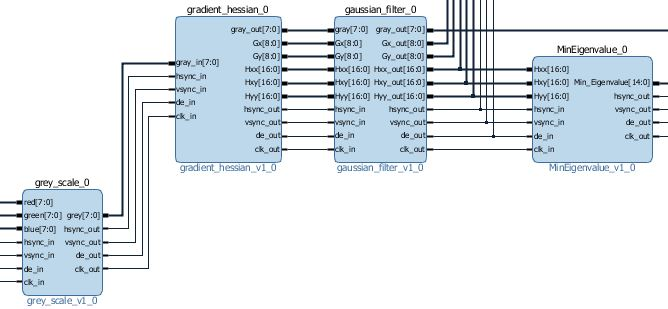
\includegraphics[width=4in]{mineig_vivado.jpg}
	\caption{Fragment schematu blokowego, realizujący wyznaczanie punktów charakterystycznych.}
	\label{fig:mineig_vivado}
\end{figure}
%TODO ref. i nie, że powyżej opisane operacje... -zrobione.

\begin{figure}[H]
	\centering
	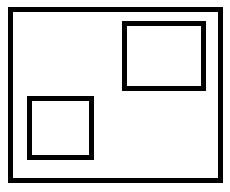
\includegraphics[width=2in]{test.jpg}
	\caption{Przykładowy obraz wejściowy.}
	\label{fig:test}
\end{figure}
%TODO ref -zrobione.

\begin{figure}[H]
	\centering
	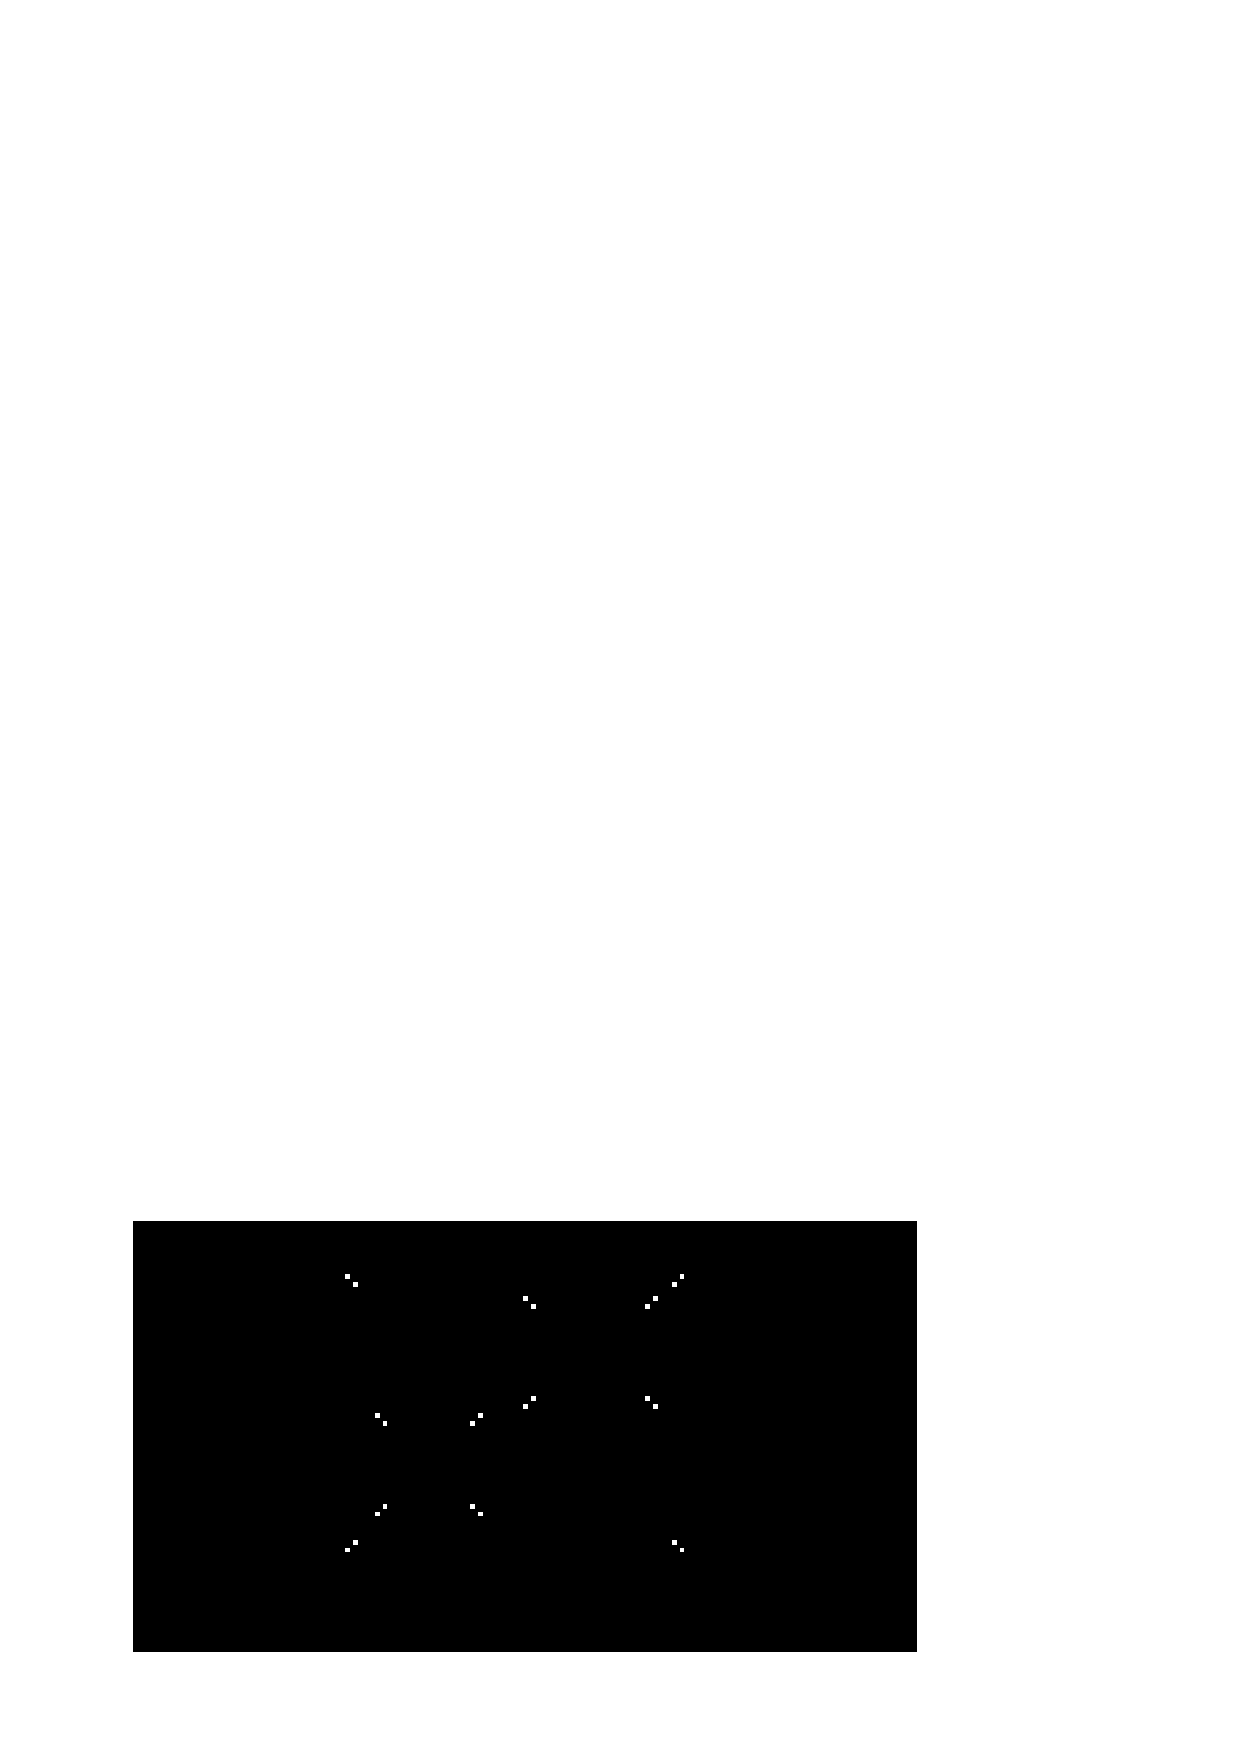
\includegraphics[width=4in]{test_out.jpg}
	\caption{Przykładowy obraz wyjściowy.}
	\label{fig:test_out}
\end{figure}
%TODO ref -zrobione.

\noindent Na rysunku \ref{fig:test} pokazano przykładowy obraz wejściowy dla którego wyznaczone zostały punkty charakterystyczne. Został on wybrany tak, by ich położenie można było bardzo łatwe do określenia (znajdują się one w rogach prostokątów).\newline
Na rysunku \ref{fig:test_out} przedstawiono obraz wyjściowy, gdy na wejście został podany obraz z rysunku \ref{fig:test}. Jasne piksele oznaczają punkty charakterystyczne. Zgodnie z przewidywaniami znajdują się one w rogach prostokątów.

\paragraph*{}
Nie udało się dokończyć implementacji algorytmu KLT. Potrzeba jeszcze zaimplementować operacje realizujące śledzenie okna wokół wybranych punktów charakterystycznych, a więc obliczające wartość przesunięcia z równania (\ref{eq:dp_klt}) oraz iteracyjne wyznaczanie przesunięcia za pomocą wspomnianego wzoru.

%TODO Zobaczymy...
\chapter{Podsumowanie}
\label{cha:podsumowanie}



% itd.
% \appendix
% \chapter{Zawartość płyty CD}
\label{cha:zawartoscplytycd}

Na załączonej płycie CD znajduje się:
\begin{itemize}
\item Tekst pracy w formacie PDF.
\item Projekt Vivado systemu z algorytmem śledzenia przez detekcję.
\item Projekt Vivado systemu z algorytmem Mean-shift.
\item Projekt Vivado z algorytmem wykrywania punktów charakterystycznych.
\item Kod \textit{MATLAB} użyty do oceny algorytmów śledzenia.
\end{itemize}
% \include{dodatekB}
% itd.

\printbibliography

\end{document}